\chapter{Evaluation and results}


\section{Datasets}


The choice of datasets of protein-ligand complexes used for statistical analysis and P2Rank model training and evaluation was strongly inspired by the datasets described in the P2Rank article \cite{p2rank1}. The structures were re-downloaded directly from PDBe, according to their PDB ID (four-character alphanumeric identifier) and chain ID (one-character identifier) used in the original datasets. It was not possible to take the original datasets as they were, since the structures were not up-to-date and the annotations downloaded from the databases (e.g. feature values) could not be mapped properly.

Downloaded datasets were further checked and filtered: Obsolete structures were replaced with their current entries, structures that do not have a corresponding UniProt record were removed, as well as  structures with the incorrect segments mapping due to the bug in PDBe (mentioned in section TODO-ODKAZ).


The resulting datasets were named identically with the original datasets:

\begin{itemize}
  \item \textbf{Chen11}
  - a smaller non-redundant dataset that was originally designed for a comparative study of ligand binding sites predictors \cite{benchmark}. It comprises at most one representative chain for every SCOP family \cite{scop} to ensure the minimal sequence similarity and maximal variability in tertiary structure. The original dataset covers 6 structural classes, 148 protein folds, 184 superfamilies and 251 families \cite{benchmark}; after re-downloading and filtering, the numbers are slightly smaller. Although this dataset is rather small, it covers wide range of non-homologous proteins. Therefore, it serves as good training dataset (P2Rank default model was trained on this dataset as well).
  
  \item \textbf{Coach420}
  - a dataset that was originally taken from a benchmark study \cite{cofactor} and used in other studies \cite{coach, p2rank1}. The non-redundant dataset harbor mix of natural and drug-like ligand molecules.
  
  \item \textbf{Joined}
  - smaller datasets from previous studies merged together in one larger dataset. It comprises a set of drug-target complexes extracted from DrugBank, DrugPort and PDB DT198\cite{dt}, a benchmark set for the validation of protein-ligand docking performance \cite{astex}, and a dataset with bound and unbound structures used for evaluation of a ligand binding sites predictor \cite{ligsite}.
  
  \item \textbf{Holo4k}
  - a large set of protein-ligand complexes used in a large-scale evaluation of four binding sites predictors \cite{holo4k}.
\end{itemize}



TODO single chain

\subsection{Ligands filtering}

\section{Statistical analysis}

TODO vymenit grafy za ty nove, hezci, lepci!

The statistical analysis of ligand binding sites properties was computed using the analysis pipeline described in TODO section 3 with default parameters. The results were collected for all the datasets, including the versions with filtered ligands. Let's set the significance level, denoted by $\alpha$, to 0.05.

Some features had to be excluded from the analysis, since the data were very sparse and the assumptions of the hypothesis tests would not be met. For example, there were only 15 lipidation sites in the whole holo4k dataset containing  857,635 residues. The excluded features are: \texttt{lipidation}, \texttt{glycosylation}, \texttt{non\_standard} and \texttt{compbias}

The \texttt{conservation} feature was computed only for the three smaller datasets and was omitted for holo4k. The computational time would be very high, as it takes 15-30 minutes on average per structure, and the dataset contains almost four thousand proteins. Nevertheless, the comparison on the other three datasets seems sufficient.

The problem with feature \texttt{variation} was that the data were missing for many structures (around 3/4) and downloading via REST API resulted in 404 Not Found error. Data are not available on the UniProt website either. This might be caused by lack of variation data from large-scale studies for some organisms. UniProt helpdesk was contacted to help to explain the issue, but unfortunately, the question was left without an answer. Nevertheless, the feature was analysed on the subset of structures where the data is available.

For some features downloaded from databases, such as \texttt{depth} or \texttt{dynamine}, there were missing data for a few structures as well. These cases were not very frequent and they most likely could not affect the analysis, so they were omitted.

Three artificial features were added for comparison and to check the validity of the tool:
\begin{itemize}
  \item \texttt{lbs} - Ligand binding sites labels (0/1). Should have the best performance of all the features, the P-value should be zero.
  \item \texttt{random\_binary} - Random binary numbers. Should not be significant.
  \item \texttt{random\_cont} - Random continuous feature with values from uniform distribution from 0 to 10.
\end{itemize}

The results for datasets without ligands filter are shown in Table~\ref{tab:pvaluesAll}. As we can see, most features appear to be statistically significant, having the P-value below the significance level $\alpha$. The results for the test features \texttt{lbs}, \texttt{random\_binary} and \texttt{random\_cont} seem to be okay. However, when looking at the histograms and plots, some results are not as expected. Let's take a look at the histogram depicted in Figure~\ref{fig:dynamine}: the distribution of \texttt{dynamine} values does not seem significantly different in binding and non-binding sites. Note that for better comparison of binding and non-binding sites (since their ratio is very unbalanced), the density is computed with respect to the number of binding or non-binding sites; the value in the histogram bin can be understood as conditional probability of getting that value when having a binding/non-binding residue.

% Please add the following required packages to your document preamble:
% \usepackage[table,xcdraw]{xcolor}
% If you use beamer only pass "xcolor=table" option, i.e. \documentclass[xcolor=table]{beamer}
\begin{table}[]
\centering
\begin{tabular}{lllll}
\hline
\textbf{}                     & \textbf{Chen11}                & \textbf{Coach420}               & \textbf{Joined}                & \textbf{Holo4k}                 \\ \hline
\textbf{lbs (test)}                  & 0                              & 0                               & 0                              & 0                               \\
\textbf{conservation}         & 0                              & 0                               & 0                              & ---                             \\
\textbf{pdbekb\_conservation} & 0                              & 0                               & 0                              & 0                               \\
\textbf{HSE\_up}              & 1.48E-266                      & 0                               & 0                              & 0                               \\
\textbf{exposure\_CN}         & 2.08E-240                      & 0                               & 0                              & 0                               \\
\textbf{depth}                & 1.63E-225                      & 3.37E-244                       & 0                              & 0                               \\
\textbf{bfactor}              & 6.57E-176                      & 1.02E-172                       & 9.03E-280                      & 0                               \\
\textbf{aa}                   & 2.43E-141                      & 4.01E-118                       & 2.09E-224                      & 0                               \\
\textbf{mol\_weight}          & 2.54E-141                      & 1.77E-117                       & 2.71E-225                      & 0                               \\
\textbf{HSE\_down}            & 4.23E-139                      & 6.18E-225                       & 0                              & 0                               \\
\textbf{hydropathy}           & 9.39E-136                      & 1.83E-118                       & 9.79E-222                      & 0                               \\
\textbf{aromaticity}          & 5.53E-79                       & 3.97E-56                        & 1.79E-102                      & 0                               \\
\textbf{H\_bond\_atoms}       & 3.59E-44                       & 2.89E-36                        & 4.50E-72                       & 0                               \\
\textbf{strand}               & 2.11E-17                       & 7.37E-32                        & 7.58E-36                       & 2.02E-252                       \\
\textbf{sec\_str}             & 2.88E-16                       & 1.57E-45                        & 4.91E-42                       & 0                               \\
\textbf{helix}                & 5.59E-06                       & 3.28E-29                        & 1.19E-26                       & 5.83E-279                       \\
\textbf{phi\_angle}           & 9.89E-06                       & 4.29E-05                        & 1.07E-07                       & 1.36E-42                        \\
\textbf{mobiDB}               & 0.0006394                      & 0.007984                        & 4.54E-06                       & 5.98E-51                        \\
\textbf{PTM}                  & 0.007131                       & 5.29E-05                        & 1.77E-15                       & 1.15E-104                       \\
\textbf{psi\_angle}           & 0.009603                       & 7.71E-16                        & 0.0009644                      & 1.30E-27                        \\
\textbf{charged}              & 0.009871                       & 4.38E-13                        & 2.99E-05                       & 2.53E-159                       \\
\textbf{dynamine}             & 0.0143                         & 0.02082                         & \cellcolor[HTML]{F54D4D}0.1595 & 1.70E-05                        \\
\textbf{efoldmine}            & 0.01699                        & 0.002727                        & 1.06E-09                       & 5.02E-07                        \\
\textbf{polarity}             & 0.02564                        & 9.01E-13                        & 3.11E-06                       & 4.18E-159                       \\
\textbf{variation*}            & \cellcolor[HTML]{F54D4D}0.1513 & \cellcolor[HTML]{F54D4D}0.07348 & \cellcolor[HTML]{F54D4D}0.698  & \cellcolor[HTML]{F54D4D}0.05166 \\
\textbf{cis\_peptide}         & \cellcolor[HTML]{F54D4D}0.2373 & 0.0001902                       & 4.44E-06                       & 3.46E-45                        \\
\textbf{disulfid}             & \cellcolor[HTML]{F54D4D}0.2753 & 1.82E-06                        & \cellcolor[HTML]{F54D4D}0.5603 & 1.71E-33                        \\
\textbf{natural\_variant}     & \cellcolor[HTML]{F54D4D}0.2793 & 0.02171                         & 2.14E-07                       & 3.39E-24                        \\
\textbf{mod\_res}             & \cellcolor[HTML]{F54D4D}0.3116 & 0.002696                        & 9.69E-05                       & 2.72E-49                        \\
\textbf{random\_cont (test)}         & \cellcolor[HTML]{F54D4D}0.4707 & \cellcolor[HTML]{F54D4D}0.706   & \cellcolor[HTML]{F54D4D}0.99   & \cellcolor[HTML]{F54D4D}0.1021  \\
\textbf{random\_binary (test)}       & \cellcolor[HTML]{F54D4D}0.5429 & \cellcolor[HTML]{F54D4D}0.922   & \cellcolor[HTML]{F54D4D}0.3561 & \cellcolor[HTML]{F54D4D}0.9322  \\
\textbf{turn}                 & \cellcolor[HTML]{F54D4D}0.8949 & 0.003081                        & \cellcolor[HTML]{F54D4D}0.7883 & 0.006317                        \\ \hline
\end{tabular}
\caption{P-values returned by hypothesis tests for individual features for all four datasets (without ligands filtering). Features are sorted according to the P-value in the first column. Values highlighted with red colour are higher that the chosen significance level $\alpha = 0.05$.\\\hspace{\textwidth}
*\texttt{variation} is computed only on the subsets of proteins for which the data were available in databases.}
\label{tab:pvaluesAll}
\end{table}

\begin{figure}[!htbp]
\centering
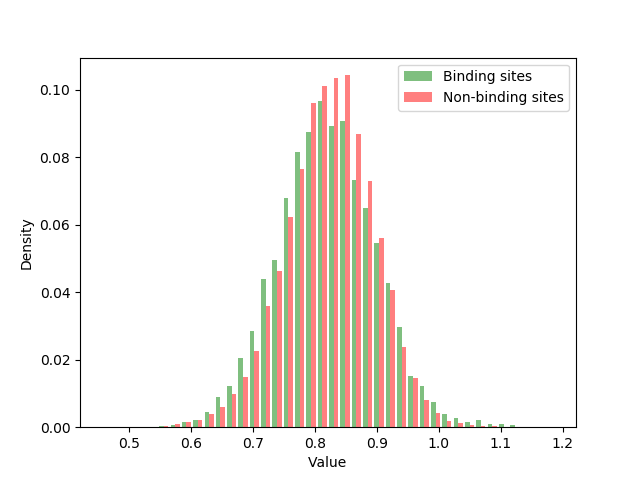
\includegraphics[width=120mm]{../img/dynamine_hist.png}
\caption{Histogram of feature \texttt{dynamine} computed on holo4k dataset. Density on the y-axis is computed with respect to the number of binding or non-binding sites. Difference in means: 0.0014; difference in variances: 0.0015.}
\label{fig:dynamine}
\end{figure}

One conspicuous thing about the Table~\ref{tab:pvaluesAll} is that, in general, the P-values are getting smaller as the dataset size grows (the datasets in the table are sorted from the smallest on the left to the largest on the right). This is referred to as the \textit{P-value problem}. For very large samples, the statistical power of hypothesis tests is higher, and causes P-value going to zero. When dealing with large samples, even the miniscule effects can become statistically significant. The test can detect subtler and more complex effects, which can be advantageous in some cases, but also misleading. It all depends on the purpose of the statistical testing. The question we should ask is not whether the results are statistically significant (which there almost always will be for large samples), but whether they are interesting for our research \cite{pvalueproblem}.

The P-value itself does not have an objective meaning and is not an unambiguous measure of evidence. The sample size hugely influences the significance, and relying only on the P-value can lead to acceptance of the hypothesis of no practical significance. Despite that, this appears to be a common practice. Lin et al. \cite{pvalueproblem} reviewed articles in two leading Information System (IS) journals and reported that 50\% of recent papers with sample sizes over 10,000 were relying on low P-values.

Let's see the P-value problem demonstated on our data. Figure~\ref{fig:pvalueDeflation} shows different speeds of P-value deflation for chosen features. At the first glance, the distributions of feature \texttt{exposure\_CN} in binding and non-binding sites differ, and sample size 25 is sufficient to get the P-value below significance level 0.05. On the other hand, \texttt{dynamine} does not seem to be relevant for the binding sites recognition, and yet, if the sample size is large enough, we get the significant result.


\begin{figure}[!htbp]
\centering
\begin{subfigure}[b]{\textwidth}
  \centering
  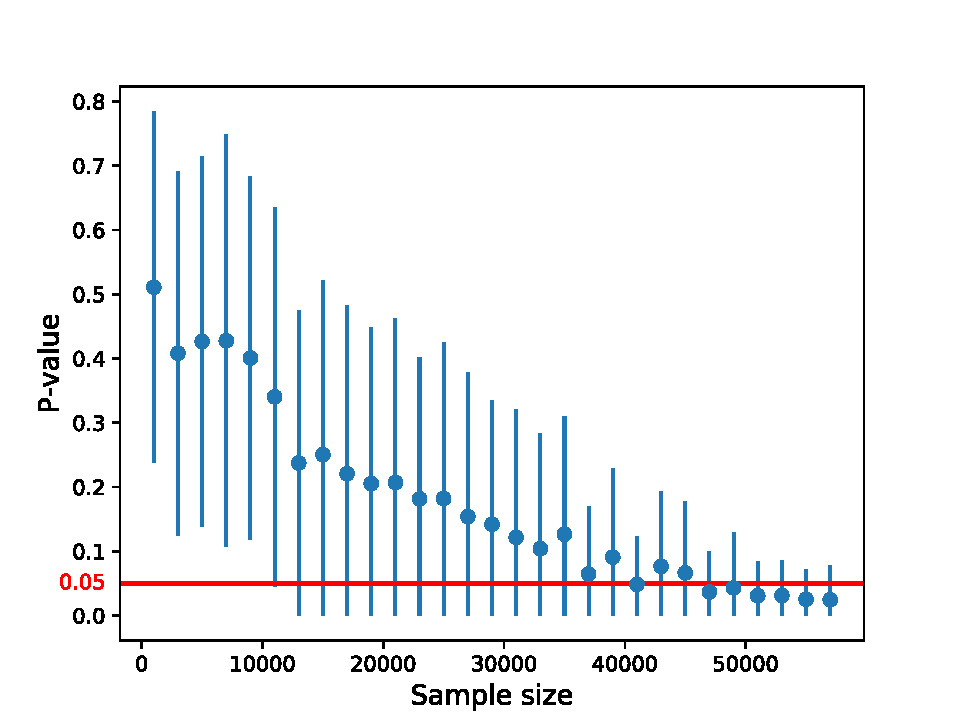
\includegraphics[width=0.475\linewidth]{../img/pValue_deflation_dynamine.pdf}%
  \hfill
  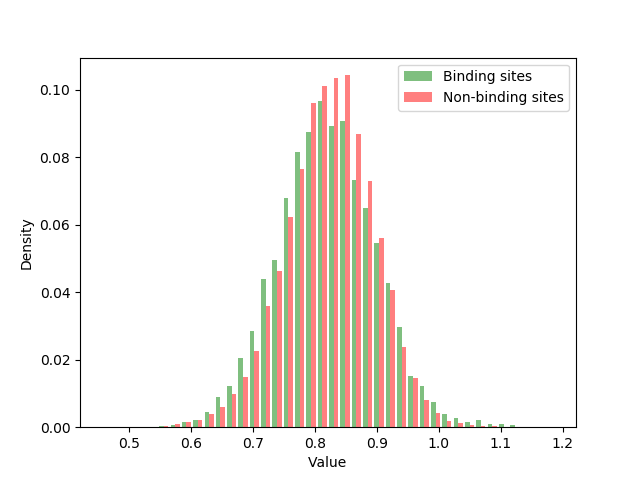
\includegraphics[width=0.475\linewidth]{../img/dynamine_hist.png}
  \caption{\texttt{dynamine}}
\end{subfigure}
\vskip\baselineskip
\begin{subfigure}[b]{\textwidth}
  \centering
  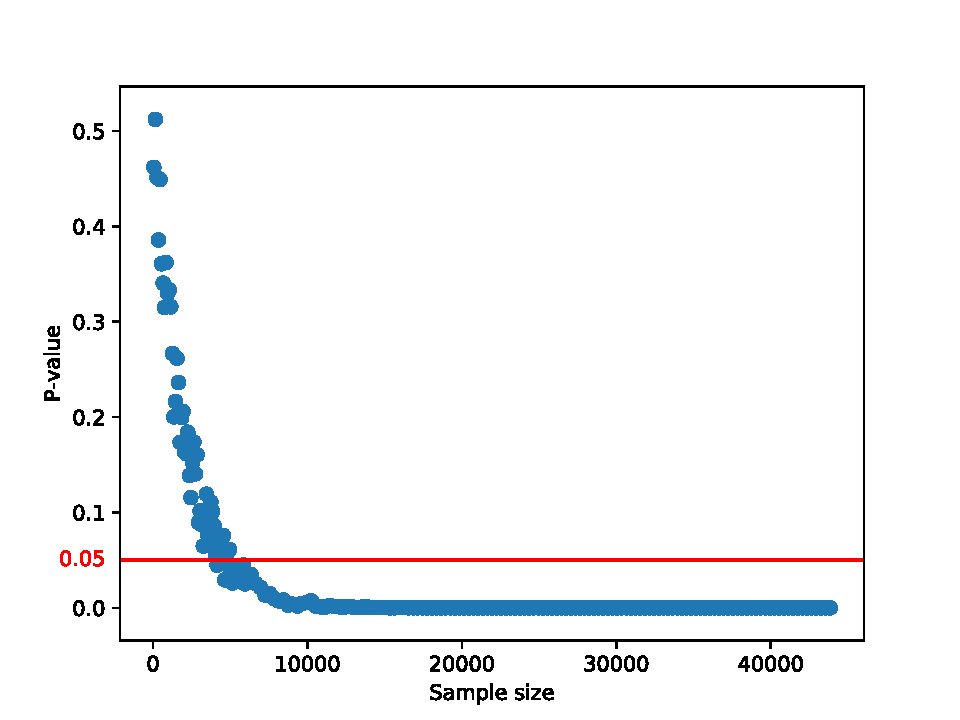
\includegraphics[width=0.475\linewidth]{../img/pValue_deflation_phi_angle.pdf}%
  \hfill
  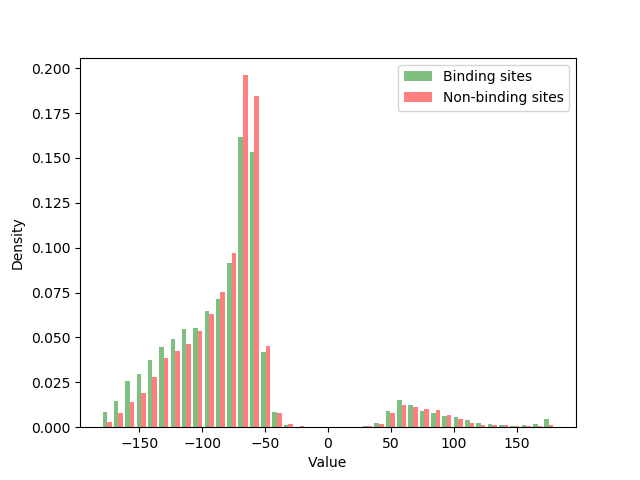
\includegraphics[width=0.475\linewidth]{../img/phi_angle_hist.png}
  \caption{\texttt{phi\_angle}}
\end{subfigure}
\vskip\baselineskip
\begin{subfigure}[b]{\textwidth}
  \centering
  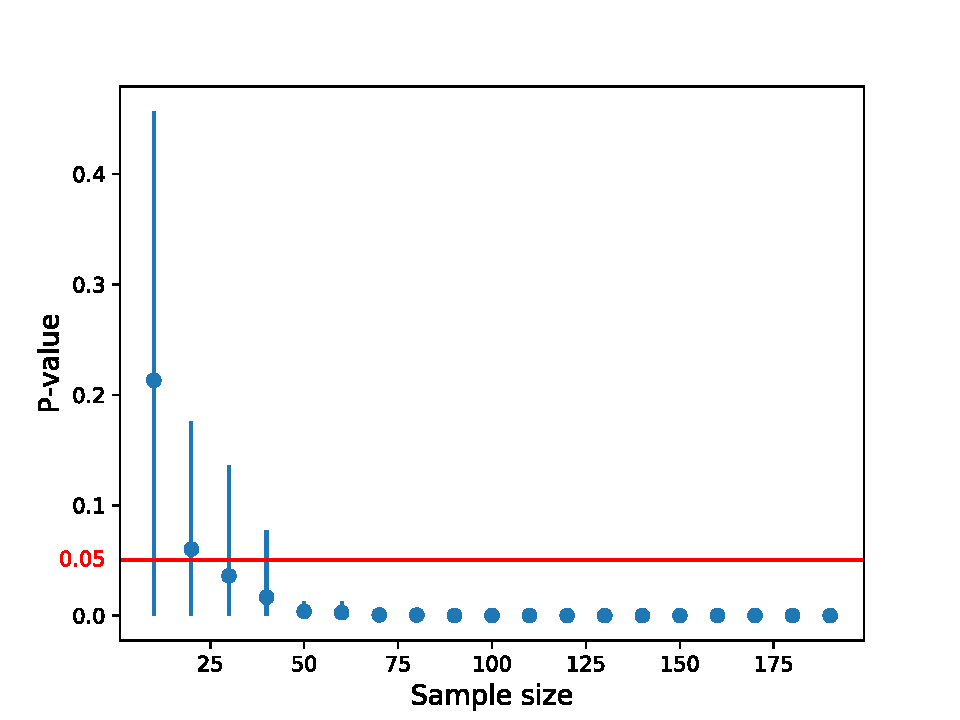
\includegraphics[width=0.475\linewidth]{../img/pValue_deflation_exposure_CN.pdf}%
  \hfill
  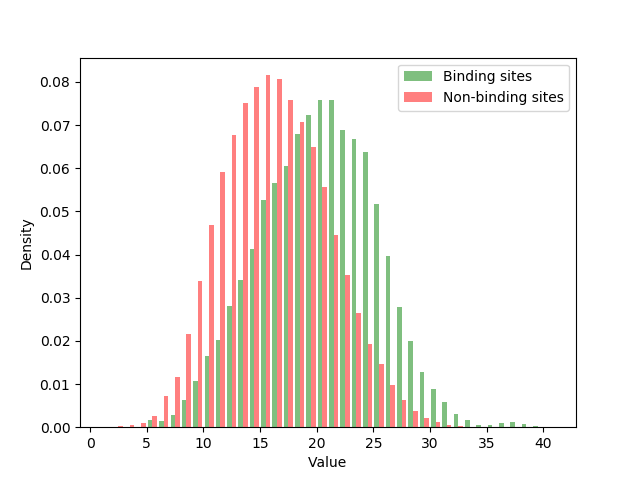
\includegraphics[width=0.475\linewidth]{../img/exposure_CN_hist.png}
  \caption{\texttt{exposure\_CN}}
\end{subfigure}
\caption{P-value deflation demonstrated on chosen features. The P-value decreases with increasing sample size. The speed of deflation is different for individual features. The y-axis shows mean P-values obtained from 100 iterations of random sampling with given sample size. The red line represents chosen significance level $\alpha=0.05$. }
\label{fig:pvalueDeflation}
\end{figure}


Therefore, the low P-values reported in Table~\ref{tab:pvaluesAll} are most likely mere artifacts of the large-sample sizes. Neverthleless, although P-value is not an objective measure of practical significance, it can be still used to compare the features relative to each other.

Another noticeable thing about Table~\ref{tab:pvaluesAll} is that the results for some features vary across datasets. Let's take a look at feature \texttt{turn}, for example. The P-value is very high for datasets Chen11 and Joined - even higher than P-values for the random features; contrarily, it is low for Coach420 and Holo4k. It is not true that the P-value would decrease with the increasing sample size. This leads to a question of how the datasets are composed, and whether they are representative samples from the whole population of proteins. Taken into consideration the way how the datasets were assembled, it is likely that some bias was introduced. The question is whether taking the whole PDB database would help to solve this issue. There probably would be the problem with redundancy of data, as close homologs and overlapping PDB entries would be included. Furthermore, the database itself is most likely a biased sample of the real world of proteins, as the tertiary structure is yet to be discovered for many of them. And most importantly, this approach would be computationally very demanding.

For the mentioned reasons, a different approach was implemented. Dataset `mix' was created by merging all four datasets together, removing a few duplicates. Random sampling without replacement was applied on this dataset, in each iteration taking a sample of 500 binding and 500 non-binding sites. 1000 iterations were computed and mean P-values were reported. The results are shown in Table~\ref{tab:pvalues500}. Note that the mean P-value cannot be understood in the original meaning of P-value. Nevertheless, the numbers provide relative comparison of the features.

The sample size of 500 was chosen for two reasons: firstly,  validity of the Central Limit Theorem needs to be assured, as described in section TODO. Lumley \textit{et al.} \cite{lumley} demonstrated that 500 is a sufficiently large sample even for extremely non-normal data. And secondly, the minimum sample size assuring the Central Limit Theorem validity should be chosen, to avoid the P-value problem. Smaller sample size would probably be sufficient for the Central Limit Theorem, as 500 is a very safe estimation. Nevertheless, the sample size could not be much smaller anyhow, since the data for some categorial features would be very sparse. Even with the sample size of 500, some features needed to be excluded from the analysis, as there was not sufficient number of positives in this smaller sample. TODO vyjmenovat je

TODO taky vyhoda, ze nebudou zavislosti mezi rezidui

% Please add the following required packages to your document preamble:
% \usepackage[table,xcdraw]{xcolor}
% If you use beamer only pass "xcolor=table" option, i.e. \documentclass[xcolor=table]{beamer}
\begin{table}[!htbp]
\centering
\begin{tabular}{llll}
\hline
                              & \textbf{no filter} & \textbf{P2Rank filter} & \textbf{MOAD filter} \\ \hline
\textbf{lbs (test)}                  & 1.33E-218          & 1.33E-218              & 1.33E-218            \\
\textbf{pdbekb\_conservation} & 3.55E-27           & 1.35E-30               & 4.43E-36             \\
\textbf{conservation}         & 1.11E-17           & 1.05E-27               & 7.86E-33             \\
\textbf{exposure\_CN}         & 4.72E-17           & 1.95E-21               & 1.30E-22             \\
\textbf{HSE\_up}              & 1.15E-14           & 2.15E-18               & 1.38E-18             \\
\textbf{depth}                & 8.00E-14           & 9.13E-16               & 2.83E-16             \\
\textbf{HSE\_down}            & 1.48E-09           & 1.59E-11               & 2.28E-11             \\
\textbf{bfactor}              & 2.56E-06           & 3.03E-08               & 3.97E-08             \\
\textbf{aa}                   & 0.006394           & 0.001172               & ---                  \\
\textbf{mol\_weight}          & ---                & 0.00129                & 0.002037             \\
\textbf{hydropathy}           & 0.00539            & 0.001376               & 0.001953             \\
\textbf{aromaticity}          & 0.02027            & 0.01516                & 0.02523              \\
\textbf{H\_bond\_atoms}       & 0.08081            & 0.02502                & 0.03019              \\
\textbf{charged}              & 0.2683             & 0.06663                & 0.08965              \\
\textbf{polarity}             & 0.2755             & 0.07131                & 0.1009               \\
\textbf{sec\_str}             & 0.133              & 0.0873                 & 0.02696              \\
\textbf{strand}               & 0.1491             & 0.1112                 & 0.04838              \\
\textbf{helix}                & 0.1361             & 0.1154                 & 0.02435              \\
\textbf{mobiDB}               & 0.3971             & 0.3844                 & 0.3653               \\
\textbf{phi\_angle}           & 0.3973             & 0.399                  & 0.3864               \\
\textbf{psi\_angle}           & 0.4213             & 0.4317                 & 0.2875               \\
\textbf{efoldmine}            & 0.4769             & 0.4373                 & 0.4839               \\
\textbf{dynamine}             & 0.4937             & 0.484                  & 0.4208               \\
\textbf{random\_cont (test)}         & 0.5029             & 0.5021                 & 0.4887               \\
\textbf{variation}            & 0.5387             & 0.5283                 & 0.5395               \\
\textbf{random\_binary (test)}       & 0.5374             & 0.5309                 & 0.5223               \\
\textbf{turn}                 & 0.5785             & 0.5982                 & 0.598                \\ \hline
\end{tabular}
\caption{Mean P-values computed from 1000 iterations of random sampling with sample size 500. Computed on dataset mix (4 datasets merged together) with three variations of ligands filtering. Features are sorted according to the P-value in the second column. Some values are missing because the assumptions of the test were not met.\\\hspace{\textwidth}
*\texttt{variation} is computed only on the subsets of proteins for which the data were available in databases.}
\label{tab:pvalues500}
\end{table}

The results for the datasets with different ligands filters does not seem to differ widely and does not reveal any additional informations. For that reason, following features analysis and computed plots will be shown only for the dataset `mix' with P2Rank ligands filter. The results obtained from the analysis pipeline for all the datasets and various sample sizes are included in the Attachments. TODO odkaz

The results for both conservation features \texttt{conservation} and \texttt{pdbekb\_conservation} turned out as expected. Sequence conservation has been used previously in many approaches for protein-ligand binding sites prediction and its importance for the prediction has been repeatedly demonstrated \cite{ligsite, cons, casp, prankweb}. The higher values of conservation for binding residues are clearly visible from the Figure~\ref{fig:conservation}.

\begin{figure}[!htbp]
\centering
\begin{subfigure}{.5\textwidth}
  \centering
  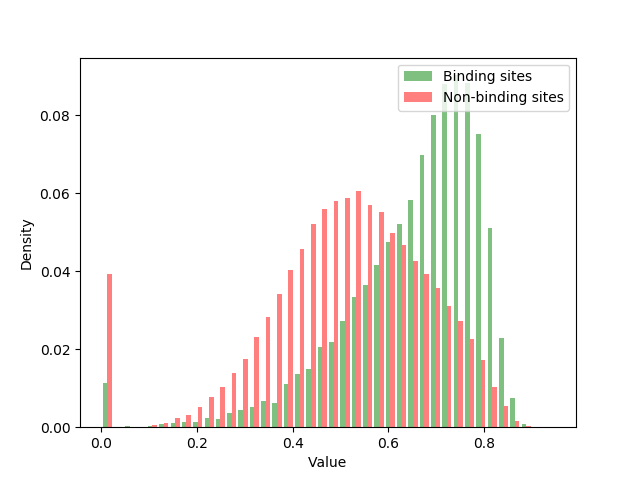
\includegraphics[width=1\linewidth]{../img/conservation_hist.png}
  \caption{\texttt{conservation}}
\end{subfigure}%
\begin{subfigure}{.5\textwidth}
  \centering
  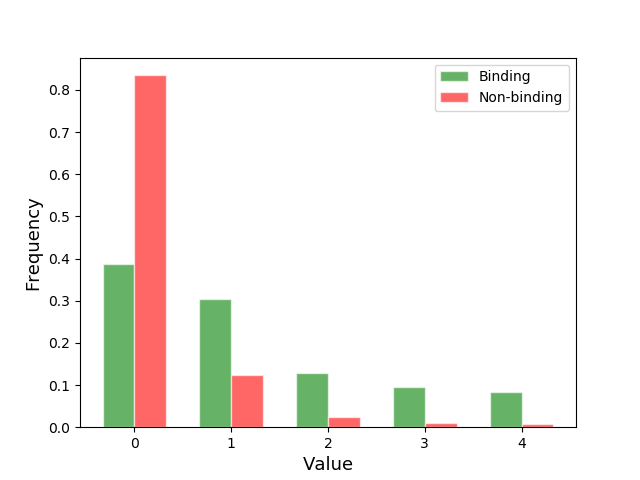
\includegraphics[width=1\linewidth]{../img/pdbekb_conservation_frequencies.png}
  \caption{\texttt{pdbekb\_conservation}}
\end{subfigure}
\caption{Higher values of conservation for binding residues demonstrated on two features: (a) continuous feature computed by the conservation pipeline, and (b) ordinal feature downloaded from PDBe-KB database.}
\label{fig:conservation}
\end{figure}

Features \texttt{HSE\_up}, \texttt{HSE\_down}, \texttt{exposure\_CN} and \texttt{depth} are closely related to the `buriedness' of the residue. Similarly as conservation, this feature was expected to be important for ligand binding sites recognition. Many binding sites are shaped as cavities, or concave pockets, on the surface of the 3D structure. The geometrical methods, such as LIGSITE \cite{ligsite} or PocketPicker \cite{pocketpicker}, as well as other approached, make use of this property. The histograms for these continuous features are depicted in Figure~\ref{fig:buriedness}


\begin{figure}[!htbp]
\centering
\begin{subfigure}{.5\textwidth}
  \centering
  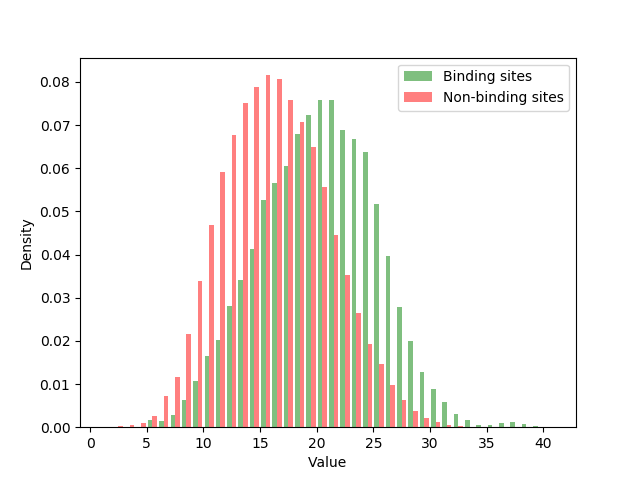
\includegraphics[width=1\linewidth]{../img/exposure_CN_hist.png}
  \caption{\texttt{exposure\_CN}}
\end{subfigure}%
\begin{subfigure}{.5\textwidth}
  \centering
  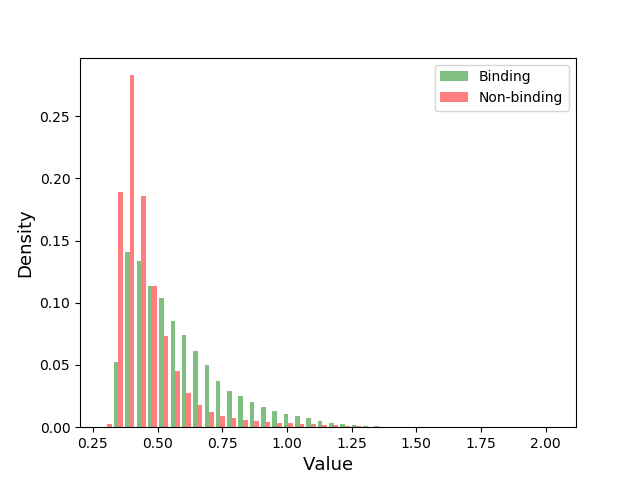
\includegraphics[width=1\linewidth]{../img/depth_hist.png}
  \caption{\texttt{depth}}
\end{subfigure}
\begin{subfigure}{.5\textwidth}
  \centering
  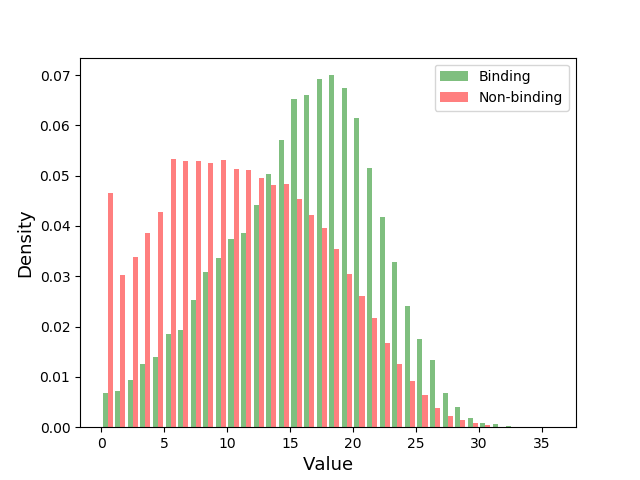
\includegraphics[width=1\linewidth]{../img/HSE_up_hist.png}
  \caption{\texttt{HSE\_up}}
\end{subfigure}%
\begin{subfigure}{.5\textwidth}
  \centering
  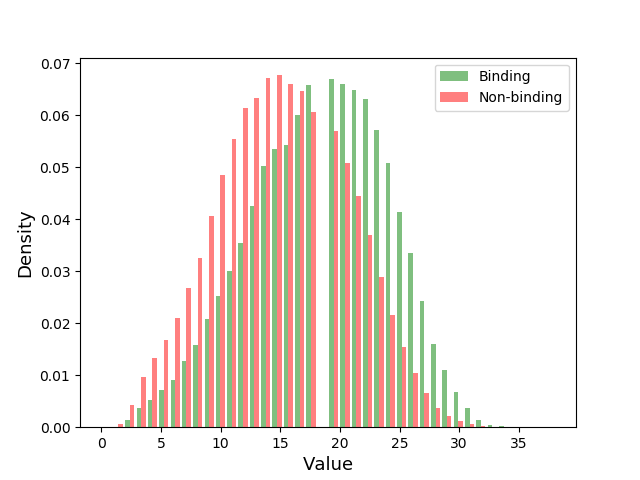
\includegraphics[width=1\linewidth]{../img/HSE_down_hist.png}
  \caption{\texttt{HSE\_down}}
\end{subfigure}
\caption{The features related with buriedness of the residue have higher values in binding sites.}
\label{fig:buriedness}
\end{figure}

The analysis reveals that binding sites have on average slightly lower B factor values (see Figure~\ref{fig:bfactor}). This suggests that binding sites are more well-ordered in general, whereas non-binding sites might have higher flexibility.

\begin{figure}[!htbp]
\centering
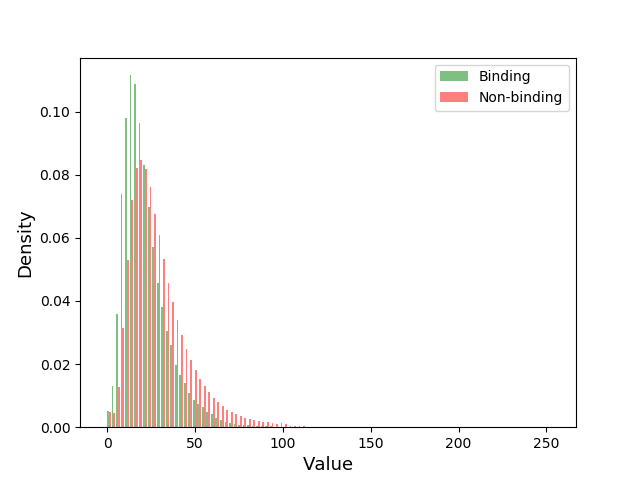
\includegraphics[width=0.7\linewidth]{../img/bfactor_hist.png}
\caption{\texttt{bfactor}: Binding sites have lower B factor values on average.}
\label{fig:bfactor}
\end{figure}

Binding and non-binding sites seem to have different residue composition. Let's take a look at Figure~\ref{fig:aa}. Cys, Trp, Phe, Tyr, Gly, His, Met and Ile all have high binding/non-binding ratios, and thus, are more likely to occur in binding sites. On the other hand, Pro, Glu, Gln, Lys and Asp disfavour binding sites. Arg, Val, Ser and Leu are very frequent in binding sites; however, they have the ratios similar to the total binding/non-binding ratio, as they are very frequent on the whole protein surface, not only in binding sites. This result is in accordance with a large-scale study that explored the composition of protein-ligand binding sites \cite{lbscomposition}. 
This is an interesting result and higher propensities of some amino acids to appear in binding sites could be used for their prediction.


\begin{figure}[!htbp]
\centering
\begin{subfigure}{\textwidth}
  \centering
  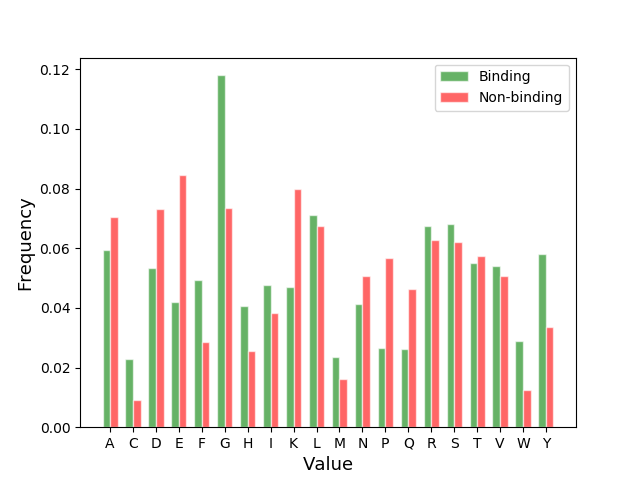
\includegraphics[width=0.7\linewidth]{../img/aa_frequencies.png}
  \caption{Frequencies of individual amino acids in binding and non-binding sites.}
\end{subfigure}
\begin{subfigure}{\textwidth}
  \centering
  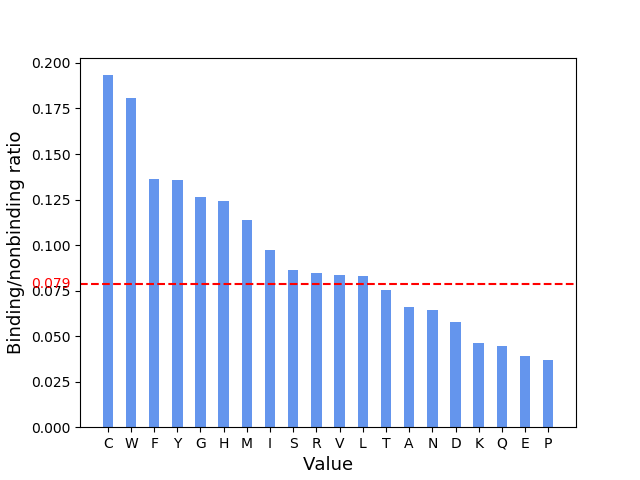
\includegraphics[width=0.7\linewidth]{../img/aa_ratios.png}
  \caption{Comparison of binding/non-binding ratios, computed as occurrences of the AA in binding sites divided by its occurrences in non-binding sites. The red line marks the total binding/non-binding ratio (total number of binding sites divided by total number of non-binding sites). High ratio means that the AA favours binding sites, and on the contrary, the low ratio indicates the tendency to occur in non-binding sites.}
\end{subfigure}
\caption{Feature \texttt{aa}.}
\label{fig:aa}
\end{figure}

TODO analyza nejakych dalsich featur?

TODO !!!!  It was discovered that high B-factor-characterized regions show a
higher average flexibility index, more pronounced average
hydrophilicity, and higher absolute net charge. - (11) Radivojac, P.; Obradovic, Z.; Smith, D. K.; Zhu, G.; Vucetic, S.;
Brown, C. J.; Lawson, J. D.; Dunker, A. K. Protein flexibility and
intrinsic disorder

TODO high-B-factor ordered regions
have a higher average flexibility index, a higher average
hydrophilicity, a higher average absolute net charge, and a
higher total charge than do either short or long disordered
regions. The low-B-factor ordered regions are significantly
enriched in hydrophobic residues and depleted in the total
number of charged residues compared to the other three
classes. 




\section{P2Rank models}

TODO evaluation metrics

The computed features were used to train new P2Rank models and analyze their practical significance. All models were trained with the same parameters as the default P2Rank model (100 trees, each grown with no depth limit using 6 features). The models were trained on the Chen11 dataset and evaluated on Coach420 dataset. The training was done with parameter \texttt{loop=10} which means that training was done 10 times, every time with different random seed, and the performance of the 10 resulting models was averaged at the end. This is important for the comparison of features importance so that the random behaviour of the random forest classifier does not have such big influence.

The features obtained by the analysis pipeline are called `csv features' in the following section, in accordance with the terminology used by P2Rank for user-defined features in csv files.

TODO ze se nektere featury vynechaly a proc: aa, secstr, variation

The performance of the baseline model (all default P2Rank features and no csv feature) was compared with the model trained on all csv features (without test features \texttt{lbs}, \texttt{random\_binary} and \texttt{random\_cont}), and the model trained with all P2Rank features and all csv features. The results are summarized in Table~\ref{tab:p2rankbaseline}. Our baseline model performs a little better in the Top-n category than the default P2Rank model described in the P2Rank article \cite{p2rank1}, which achieves the success rate of 72\%. This can be caused by  slightly different datasets, as described in Section TODO, or simply by the random behaviour of the classifier.

The performance of the model trained on the csv features is inferior to the baseline model, but surprisingly, the difference is very small. The reason probably is that many features used by P2Rank are identical or very similar to the new csv features. P2Rank already used B factor, amino acid properties, buriedness and other properties for training, and csv features evidently does not contribute with much new information. That is visible on the model with both csv and P2Rank features: the performance is superior only by 1.5\%. Moreover, csv features are mutually correlated, as well as P2Rank features. 

\begin{table}[]
\centering
\begin{tabular}{lll}
\hline
\textbf{}                                 & Top-n & Top-(n+2) \\ \hline
\textbf{P2Rank features (baseline model)} & 73.6  & 78        \\
\textbf{csv features}                     & 70.7  & 73.9      \\
\textbf{P2Rank + csv features}            & 75.1  & 77.5      \\ \hline
\end{tabular}
\caption{Comparison of the performance of models with different sets of features.}
\label{tab:p2rankbaseline}
\end{table}

Let's take a look at how the csv features help to improve the performance when adding only one of them at a time. Table~\ref{tab:p2rankCSV} summarizes the results of training one model per feature, with all P2Rank default features plus given csv feature. Models with features \texttt{pdbekb\_conservation} and \texttt{conservation} are clearly superior to the baseline model.  There are other features that perform better than the baseline model by tenths of percent; nevertheless, this difference is too small to proclaim the results significant. Although there are features that are enriched in binding sites, as has been shown previously, they do not help to improve P2Rank performance, probably due to the correlations and recurrence of the same features.

\begin{table}[]
\centering
\begin{tabular}{lll}
\hline
                              & Top-n & Top-(n+2) \\ \hline
\textbf{lbs (test)}                  & 90.2  & 90.5      \\
\textbf{pdbekb\_conservation} & 78.9  & 81.6      \\
\textbf{conservation}         & 76.8  & 79.8      \\
\textbf{HSE\_down}            & 74.1  & 78.6      \\
\textbf{helix}                & 73.6  & 78.6      \\
\textbf{psi\_angle}           & 74.3  & 78.4      \\
\textbf{depth}                & 73.2  & 78.4      \\
\textbf{turn}                 & 73.8  & 78.3      \\
\textbf{HSE\_up}              & 73.6  & 78.2      \\
\textbf{strand}               & 73.6  & 78.2      \\
\textbf{mol\_weight}          & 73.5  & 78.2      \\
\textbf{aromaticity}          & 73.6  & 78.1      \\
\textbf{dynamine}             & 73.6  & 78.1      \\
\textbf{charged}              & 73.5  & 78.1      \\
\textbf{H\_bond\_atoms}       & 73.5  & 78.1      \\
\textbf{efoldmine}            & 74.1  & 78        \\
\textbf{phi\_angle}           & 73.8  & 78        \\
\textbf{mobiDB}               & 73.6  & 78        \\
\textbf{exposure\_CN}         & 73.5  & 78        \\
\textbf{hydropathy}           & 73.3  & 77.8      \\
\textbf{bfactor}              & 73    & 77.5      \\ \hline
\end{tabular}
\caption{Performance of models trained with all P2Rank features plus one extra csv feature at a time. The features are sorted according to the performance in Top-(n+2) category.}
\label{tab:p2rankCSV}
\end{table}

In another experiment, all P2Rank features were switched off and the models were trained with csv features only, one at a time. The performances are of course wery poor, but it gives us the relative comparison of csv features, without the effect of correlation with existing P2Rank features. Table~\ref{tab:p2rankCSVOne}


\begin{table}[]
\centering
\begin{tabular}{lll}
\hline
                              & Top-n & Top-(n+2) \\ \hline
\textbf{lbs (test)}                  & 88.3  & 90        \\
\textbf{pdbekb\_conservation} & 57.1  & 71.9      \\
\textbf{HSE\_up}              & 36.7  & 52.1      \\
\textbf{conservation}         & 34    & 49.7      \\
\textbf{exposure\_CN}         & 30.8  & 44.7      \\
\textbf{HSE\_down}            & 28.2  & 41.8      \\
\textbf{depth}                & 25.5  & 37.5      \\
\textbf{aromaticity}          & 14.3  & 25.5      \\
\textbf{dynamine}             & 10.6  & 17.7      \\
\textbf{phi\_angle}           & 8.7   & 16.3      \\
\textbf{hydropathy}           & 10.7  & 16        \\
\textbf{mol\_weight}          & 8.4   & 15.7      \\
\textbf{random\_cont (test)}         & 8.2   & 14.1      \\
\textbf{efoldmine}            & 7.2   & 13.5      \\
\textbf{strand}               & 6.3   & 10.9      \\
\textbf{random\_binary (test)}       & 7     & 10.7      \\
\textbf{psi\_angle}           & 5.8   & 9.8       \\
\textbf{bfactor}              & 4.2   & 6.1       \\
\textbf{helix}                & 3.9   & 6         \\
\textbf{charged}              & 3.6   & 5         \\
\textbf{H\_bond\_atoms}       & 3.3   & 4.9       \\
\textbf{mobiDB}               & 2.4   & 4.7       \\
\textbf{turn}                 & 0     & 0         \\ \hline
\end{tabular}
\caption{Sorted by sec col}
\label{tab:p2rankCSVOne}
\end{table}

